\section{Spiegelnde Reflexion}
\begin{center}
 \psset{Alpha=175,Beta=10}
 \begin{pspicture}(-2,0)(4,4)
  \pstThreeDSquare(0,0,0)(4,0,0)(0,4,0)
  \pstThreeDPut(3,2,3){\rnode{A}{Auge}}
  \pstThreeDPut(-1,2,3){
\includegraphics[width=0.6cm]{bulb.eps}}
  \pstThreeDNode(2,2,0){mitte}
  \ncline[linestyle=dashed]{mitte}{A}
  \pstThreeDLine{->}(2,2,0)(1,2,1)\pstThreeDPut(0.8,2,1.2){$L$}
  \pstThreeDLine[linestyle=dashed]{->}(2,2,0)(3,2,1)\pstThreeDPut(3.2,2,1.2){$L'$}
  \pstThreeDLine{->}(2,2,0)(2.447,2,1.342)\pstThreeDPut(2.3,2,1.6){$A$}
  \pstThreeDLine{->}(2,2,0)(2,2,1.414)\pstThreeDPut(2,2,1.6){$N$}
  \pstThreeDCircle[beginAngle=0,endAngle=-45](2,2,0)(0,0,0.8)(1.2,0,0)
  \pstThreeDPut(1.8,2,0.5){$\theta$}
  \pstThreeDCircle[beginAngle=0,endAngle=45](2,2,0)(0,0,0.8)(2.8,0,0)
  \pstThreeDPut(2.2,2,0.5){$\theta$}
  \pstThreeDCircle[beginAngle=18.43,endAngle=45](2,2,0)(0,0,1)(3,0,0)
  \pstThreeDPut(2.7,2,1.1){$\alpha$}
 \end{pspicture}
\end{center}

$L'$ ist der an $N$ gespiegelte Vektor, die der "`idealen Spiegelung"'
\[\alpha = \measuredangle(A,L')\]
Modell von \textsc{Bui-Tong Phong}: Intensität ist proportional zu $\cos^n \alpha$
\begin{center}
 \psset{xunit=4.712,yunit=3,showorigin=false,algebraic=false,labels=none}
 \begin{pspicture}(-1.1,-0.1)(1.1,1.2)
  \psaxes{<->}(0,0)(-1.1,-0.1)(1.1,1.2)
  \psplot[unit=3,linecolor=red]{-1.57}{1.57}{x 180 mul 3.141592654 div cos}
  \psplot[unit=3,linecolor=red]{-1.57}{1.57}{x 180 mul 3.141592654 div cos 10 exp}
  \psplot[unit=3,plotpoints=500,linecolor=red]{-1.57}{1.57}{x 180 mul 3.141592654 div cos 50 exp}
  \psplot[unit=3,plotpoints=500,linecolor=red]{-1.57}{1.57}{x 180 mul 3.141592654 div cos 1000 exp}
  \rput[bl](0.1,1.1){$\cos^n \alpha$}
  \rput[tc](1,-0.2){$\frac{\pi}{2}$}
  \rput[tc](-1,-0.2){$-\frac{\pi}{2}$}
  \psset{unit=3}
  \uput{5pt}[45](0.785,0.707){$n = 1$}
  \uput{5pt}[28.05](0.393,0.452){$n = 10$}
  \uput{5pt}[28.05](0.2,0.3){$n = 50$}
  \uput{5pt}[20](0.05,0.1){$n = \infty$}
 \end{pspicture}
\end{center}
\begin{center}
 \psset{Alpha=170,Beta=20}
 \begin{pspicture}(-2,-3)(4,4.5)
  \pstThreeDPut(-1,2,-3){\rput{180}{
\includegraphics[width=0.6cm]{bulb.eps}}}
  \pstThreeDLine[linecolor=yellow](-1,2,-3)(2,2,0)
  \pstThreeDSquare(0,0,0)(4,0,0)(0,4,0)
  \pstThreeDPut(5,2,3){\rnode{A}{Auge}}
  \pstThreeDPut(-1,2,3){
\includegraphics[width=0.6cm]{bulb.eps}}
  \pstThreeDLine[linecolor=yellow](-1,2,3)(2,2,0)
  \pstThreeDNode(2,2,0){mittig}
  \pstThreeDNode(2.433,2.25,0){30}
  \pstThreeDNode(2.433,1.75,0){90}
  \pstThreeDNode(2,2.5,0){150}
  \pstThreeDNode(1.567,2.25,0){210}
  \pstThreeDNode(1.567,1.75,0){270}
  \pstThreeDNode(2,1.5,0){330}
  \ncline[linecolor=red]{A}{mittig}
  \pstThreeDDot(2,2,0)
  \ncline[linewidth=0.2px]{A}{30}
  \ncline[linewidth=0.2px]{A}{90}
  \ncline[linewidth=0.2px]{A}{150}
  \ncline[linewidth=0.2px]{A}{210}
  \ncline[linewidth=0.2px]{A}{270}
  \ncline[linewidth=0.2px]{A}{330}
  \rput(5,0){\rnode{a0}{$\alpha = 0$}}
  \pstThreeDNode(2.5,2,0.5){a0_a}
  \ncline{->}{a0}{a0_a}
  \rput(2,2){$\alpha > 0$}
 \end{pspicture}
 \hspace{2cm}
 \begin{pspicture}(0,0)(4,4.5)
  \rput(2,4.25){Bild aus Sicht des Auges}
  \psframe(0,0)(4,4)
  \rput{180}(2,2){
\includegraphics[width=0.35cm]{bulb.eps}}
  \pspolygon(0.5,1)(1.5,2.5)(2.5,2.5)(3.5,1)
 \end{pspicture}

\end{center}
Formel für spiegelnde Reflexion:
\[I^X = I^X_L \cdot \frac{1}{C_0 + C_1 r + C_2 r^2} \cdot K_S \cdot \cos^n \alpha,\qquad X = R, G, \text{ oder } B\]
\begin{align*}
	I_L...\ & \text{Intensität der Lichtquelle $(I_L^R, I_L^G, I_L^B)$}\\
	\frac{1}{C_0 + C_1 r + C_2 r^2}...\ & \text{Abhängigkeit von der Entfernung der Lichtquelle}\\
	K_S...\ & \text{spiegelnde Reflexionskoeffizient \emph{unabhängig von der Farbe!}}\\
	n...\ & \text{Exponent: gibt an wie glatt die Spiegelung ist}\\
	\frac{1}{C_0 + C_1 r + C_2 r^2}...\ & \text{Abhängigkeit von der Entfernung der Lichtquelle}\\
	I^R, I^G, I^B...\ & \text{Ergebnis-Intensität aus Sicht des Auges}\\
\end{align*}
\begin{center}
 \begin{pspicture}(0,0)(3,2.5)
  \rput[l](3,2){$\|L\| = \|N\| = \|A\| = 1$}
  \psline{->}(1.5,0)(1.5,2)
  \uput{3pt}[90](1.5,2){$N$}
  \psline{->}(1.5,0)(3.232,1)
  \uput{3pt}[30](3.232,1){$L'$}
  \psline{->}(1.5,0)(-0.232,1)
  \uput{3pt}[150](-0.232,1){$L$}
  \psline[linestyle=dashed](-0.232,1)(3.232,1)
  \psline{->}(1.5,0)(-0.232,1)
  \uput{3pt}[0](1.5,0.5){$L_0$}
  \psline{->}(1.45,1.1)(-0.232,1.1)
  \psline{->}(1.55,1.1)(3.232,1.1)
 \end{pspicture}
\end{center}
\begin{align*}
 L_0&...\ \text{Projektion von $L$ auf $N$}\\
    &= \langle L, N \rangle \cdot N\\
 L' &= -(L-L_0) + L_0 = 2L_0 - L, \|L'\|=1\\
 \cos \alpha &= \langle A, L' \rangle =  \langle A, 2L_0 \rangle -  \langle A, L \rangle\\
  &= 2  \langle L, N \rangle \langle N, A \rangle -  \langle A, L \rangle\\
	&= \cos \alpha
\end{align*}
\paragraph*{Näherungsmodell} (einfacher zu rechnen)\\
$H$ der Vektor, der symmetrisch zwischen $A$ und $L$ liegt.
\begin{align*}
 H_0 &= A + L & H &= \frac{H_0}{\|H_0\|} 
\end{align*}
Statt $\cos \alpha$ nimmt man $\cos \beta, \beta = \measuredangle(H,N)$
\[\cos \beta = \langle H, B \rangle \qquad \beta = 0 \Leftrightarrow \alpha = 0\]
\begin{center}
 \psset{unit=3cm}
 \begin{pspicture}(-1,0)(1,1.1)
  \psline(-1,0)(1,0)
  \SpecialCoor
  \psline{->}(0,0)(1;90)
  \uput{3pt}[90](1;90){$N$}
  \psline{->}(0,0)(1;160)
  \uput{3pt}[160](1;160){$L$}
  \psline[linestyle=dashed]{->}(0,0)(1;20)
  \uput{3pt}[20](1;20){$L'$}
  \psline{->}(0,0)(1;60)
  \uput{3pt}[60](1;60){$A$}
  \psline{->}(0,0)(1;110)
  \uput{3pt}[110](1;110){$H$}
  \psline(0.25;135)(0.35;135)
  \psarc(0,0){0.3}{110}{160}
  \psline(0.2;85)(0.3;85)
  \psarc(0,0){0.25}{60}{110}
  \psarc(0,0){0.8}{90}{110}
  \uput{3pt}[100](0.8;100){$\beta$}
  \psarc(0,0){0.8}{20}{60}
  \uput{3pt}[40](0.8;40){$\alpha$}
 \end{pspicture}
\end{center}
$\beta = \frac{\alpha}{2}$, wenn $L, N, A$ in einer Ebene liegen. Im Raum ist das nicht immer der Fall.

\section{Gesamtbeleuchtung}
\begin{itemize}
 \item mehrere Lichtquellen an bestimmten Orten (bzw. aus bestimmten Richtungen) mit Intensität $I_L^R, I_L^G, I_L^B$
 \item eine diffuse Lichtquelle mit Intensität $I_D^R, I_D^G, I_D^B$
\end{itemize}
Für jede Fläche:
\begin{itemize}
 \item diffuse Reflexionskoeffizienten $K_D^R, K_D^G, K_D^B$
 \item spiegelnde Reflexionskoeffizienten $K_S$, Exponent $n$
 \item möglicherweise eine Eigenleuchtintensität $I_E^R, I_E^G, I_E^B$ (z. B. Leuchtschirm, glühendes Ofenrohr,
									flächig leuchtende Lichtquelle)
\end{itemize}
Für jedes Flächenstück addiert man alle Beleuchtungskomponennten zusammen (falls die Fäche sichtbar vom Auge ist).
\begin{align*}
 I^R &= \sum \text{diffuse Reflexionen von allen Lichtquellen, die das Flächenstück beleuchten.} \\
	& \qquad + \text{spiegelnde Reflexionen von allen Lichtquellen, die das Flächenstück beleuchten.} \\
	& \qquad + I_{L,E}^R \cdot K^R_E
\end{align*}
analog für $I^G, I^B$
\begin{center}
 \psset{Alpha=170,Beta=20}
 \begin{pspicture}(0,0)(4,3)
  \pstThreeDSquare(0,0,0)(4,0,0)(0,4,0)
  \pstThreeDDot(0,2,2)
  \pstThreeDSquare(1,0.2,0)(0.2,0,0)(0,0.2,0)
  \pstThreeDSquare(1.4,1.5,0)(0.2,0,0)(0,0.2,0)
  \pstThreeDSquare(2,3,0)(0.2,0,0)(0,0.2,0)
  \pstThreeDSquare(3,2,0)(0.2,0,0)(0,0.2,0)
  \pstThreeDLine(0,2,2)(1.1,0.3,0)
  \pstThreeDLine(0,2,2)(1.5,1.6,0)
  \pstThreeDLine(0,2,2)(2.1,3.1,0)
  \pstThreeDLine(0,2,2)(3.1,2.1,0)
 \end{pspicture}
\end{center}
eigentlich liefert die Rechnung in jedem Punkt der Fläche ein anderes Ergebnis.
\paragraph*{Problem} Die Intensität kann in einzelnen Punkten des Bildes $> 1$ werden.
2 Möglichkeiten
\begin{enumerate}
 \item herunterskalieren aller Werte\\
	z. B. $(r;g;b) = (3;1;0{,}5) \to \left(1,\frac{1}{3},\frac{1}{6}\right)$
 \item zu große Werte werden auf 1 gesetzt (dadurch können auch Farben verfälscht werden)\\
	z. B. $(r;g;b) = \underset{\text{(sehr rotes orange)}}{(3;1;0{,}5)} \to \underset{\text{(helles gelb)}}{(1,1,0{,}5)}$
\end{enumerate}

\section{Schattierung (Shading)}
Alle folgenden Rechnungen in Weltkoordinaten
\Defi Unter \emph{Shading} versteht man die Anwendung der Beleuchtungsregeln auf jeden Punkt einer Fläche, sodass
	sich eine abgestufte Farbverteilung ergibt, die realistisch aussieht.
	\begin{center}
	\begin{pspicture}(0,0)(8,3)
	\rput(1.5,1.5){
\includegraphics[height=3cm]{polysphere.eps}}
	%http://web.gin.cz/trahern/glTest-wire.gif
	\rput(4,1.5){$\stackrel{?}\Longrightarrow$}
	\rput(6.5,1.5){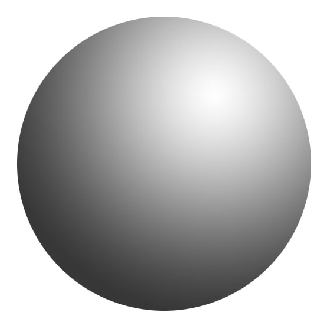
\includegraphics[height=3cm]{sphere.eps}}
	% http://www.keetee.com/downloads/sphere.jpg
	\end{pspicture}
	\end{center}
	\begin{itemize}
	 \item Gekrümmte Flächen können durch ein genügend feines \emph{Dreiecks}netz (oder Vierecksnetz) approximiert werden.
	 \item Große flache Flächen können in kleinere Dreicke zerlegt werden. 
	\end{itemize}
	\textsc{Gouraud}-Schattierung für ein Dreiecksnetz:
	\begin{itemize}
	 \item Berechne die Beleuchtung für jede Ecke eines Dreiecks , mit einem Normalvektor, der für jede Ecke fest
		ist (unabhängig von dem Dreieck zu dem es gehört). z. B. der Normalvektor der glatten Fläche, die durch
		das Dreiecksnetz approximiert wird.
		\begin{center}
		 \begin{pspicture}(0,0)(2.5,2.5)
		  \psdot(0.75,0)
		  \psdot(0,1.25)
		  \psdot(1.5,1.5)
		  \pspolygon(0.75,0)(0,1.25)(1.5,1.5)
		  \psline(2,2.25)(1.5,1.5)(2.5,1.75)
		  \psline{->}(2,0.5)(1,2.5)
		 \end{pspicture}
		\end{center}
	 \item Interpoliere die Beleuchtung linear auf jedem Dreieck
		\begin{center}
		 \begin{pspicture}(0,0)(2,2)
		  \psaxes[labels=none,ticks=none]{->}(0,0)(0,0)(2,2)
		  \psdot(0.5,0.5)\uput{3pt}[-150](0.5,0.5){5}
		  \psdot(1.5,0.5)\uput{3pt}[-30](1.5,0.5){2}
		  \psdot(1,1.5)\uput{3pt}[90](1,1.5){7}
		  \pspolygon(0.5,0.5)(1.5,0.5)(1,1.5)
		 \end{pspicture}
		\end{center}
		\[f(x,y) = ax + by + c\]
	\end{itemize}
	Die Gouraud-Schattierung, versagt z. B. bei Glanzlichtern (können verschwinden oder unnatürlich vergrößert
	werden) und sehr großen Flächen:
	\begin{center}
		\psset{Alpha=170,Beta=20}
		\begin{pspicture}(0,0)(4,3)
			\pstThreeDSquare[fillstyle=solid,fillcolor=gray](0,0,0)(4,0,0)(0,4,0)
			\pstThreeDCircle[fillstyle=solid,fillcolor=lgray,linestyle=none](2,2,0)(0.5,0,0)(0,0.5,0)
			\pstThreeDLine(4,0,0)(0,4,0)
			\pstThreeDPut(2,2,2.5){\rput{180}{
\includegraphics[width=0.6cm]{bulb.eps}}}
			\pstThreeDPut(2.5,2.5,0.1){hell?}
			\pstThreeDPut(4,0,-0.3){dunkel}
			\pstThreeDPut(0,0,-0.3){dunkel}
			\pstThreeDPut(0,4,0.3){dunkel}
			\pstThreeDPut(4,4,0.3){dunkel}
			\pstThreeDLine[linecolor=red]{->}(4,0,0)(4,2,0)
			\pstThreeDLine[linecolor=red]{->}(4,0,0)(2,0,0)
			\pstThreeDLine[linecolor=red]{->}(4,0,0)(2,2,0)
			\pstThreeDLine[linecolor=red]{->}(4,4,0)(4,2,0)
			\pstThreeDLine[linecolor=red]{->}(4,4,0)(2,4,0)
			\pstThreeDLine[linecolor=red]{->}(0,4,0)(2,2,0)
			\pstThreeDLine[linecolor=red]{->}(0,0,0)(2,0,0)
			\pstThreeDLine[linecolor=red]{->}(0,0,0)(0,2,0)
			\pstThreeDLine[linecolor=red]{->}(0,4,0)(0,2,0)
			\pstThreeDLine[linecolor=red]{->}(0,4,0)(2,4,0)
			\pstThreeDDot(0,0,0)
			\pstThreeDDot(4,0,0)
			\pstThreeDDot(0,4,0)
			\pstThreeDDot(4,4,0)
		\end{pspicture}
	\end{center}
	\textsc{Phong}-Schattierung:\\
	$\cancel{\text{diffuse Lichtquelle}}$ \emph{Umgebungslicht} (ambient light)






